\documentclass{article}
\usepackage{graphicx} % Required for inserting images
\usepackage{amsmath}
\usepackage{amsfonts}
\usepackage{comment}
\usepackage{microtype}
\usepackage{bm}
\usepackage{multicol}

\usepackage{mathtools}
\DeclarePairedDelimiter\bra{\langle}{\rvert}
\DeclarePairedDelimiter\ket{\lvert}{\rangle}
\DeclarePairedDelimiterX\braket[2]{\langle}{\rangle}{#1\delimsize\vert\mathopen{}#2}
\newcommand*\diff{\mathop{}\!\mathrm{d}}
\DeclarePairedDelimiterX\expval[3]{\langle}{\rangle}%
{#1\delimsize\vert\mathopen{}#2\delimsize\vert\mathopen{}#3}
\newcommand\HF{\ensuremath{\mathrm{HF}}}

\usepackage{hyperref}
\usepackage{xcolor}
\hypersetup{ % this is just my personal choice, feel free to change things
    colorlinks,
    linkcolor={red!50!black},
    citecolor={blue!50!black},
    urlcolor={blue!80!black},
}

% \usepackage[offset=1.2em,sep=0.3em]{simpler-wick}
\usepackage{simpler-wick}

\usepackage{enumerate}
\usepackage[shortlabels]{enumitem}
\usepackage{booktabs}
\usepackage{tikz}

\renewcommand\thesection{Exercise \arabic{section})}  % chktex 9 % chktex 10 % tex-fmt: skip
\renewcommand\thesubsection{Solution} % tex-fmt: skip
\renewcommand\thesubsubsection{\arabic{subsection}.\arabic{subsubsection})} % chktex 9 % chktex 10 % tex-fmt: skip

\title{
    Second midterm FYS4480\\
    Quantum mechanics for many-particle systems
}
\author{August Femtehjell \& Oskar Idland}
\date{November 2024}

\begin{document}

\maketitle

\section*{Introduction}
We present a simplified Hamiltonian consisting of an unperturbed Hamiltonian and a so-called pairing interaction term.
It is a model which to a large extent mimicks some central features of atomic nuclei, certain atoms and systems which exhibit superfluiditity or superconductivity.
To study this system, we will use a mix of many-body perturbation theory (MBPT), Hartree-Fock (HF) theory and full configuration interaction (FCI) theory.
The latter will also provide us with the exact answer.
When setting up the Hamiltonian matrix you will need to solve an eigenvalue problem.

We define first the Hamiltonian, with a definition of the model space and the single-particle basis.
Thereafter, we present the various exercises.

The Hamiltonian acting in the complete Hilbert space (usually infinite dimensional) consists of an unperturbed one-body part, $\hat{H}_0$, and a perturbation $\hat{V}$.
We limit ourselves to at most two-body interactions, our Hamiltonian is then represented by the following operators
\begin{equation*}
    \hat{H} = \sum_{\alpha\beta} \langle \alpha \lvert h_0 \rvert \beta \rangle a_{\alpha}^{\dagger} a_{\beta}
    + \frac{1}{4} \sum_{\alpha\beta\gamma\delta} \langle
    \alpha \beta \lvert V \rvert \gamma\delta
    \rangle
    a_{\alpha}^{\dagger} a_{\beta}^{\dagger} a_{\delta} a_{\gamma},
\end{equation*}
where $a_{\alpha}^{\dagger}$ and $a_{\alpha}$ etc.~are standard fermion creation and annihilation operators, respectively, and
$\alpha\beta\gamma\delta$ represent all possible single-particle quantum numbers.
The full single-particle space is defined by the completeness relation $\hat{{\bf 1}} = \sum_{\alpha
= 1}^{\infty} \lvert \alpha \rangle \langle \alpha \rvert$.
In our calculations we will let the single-particle states $\lvert \alpha \rangle$ be eigenfunctions of the one-particle operator $\hat{h}_0$.
Note that the two-body part of the Hamiltonian contains anti-symmetrized matrix elements.

The above Hamiltonian acts in turn on various many-body Slater determinants constructed from the single-basis defined by the one-body operator $\hat{h}_0$.
As an example, the two-particle model space $\mathcal{P}$ is defined by an operator
\begin{equation*}
    \hat{P} = \sum_{\alpha\beta =1}^{m} \lvert \alpha\beta \rangle \langle \alpha\beta \rvert,
\end{equation*}
where we assume that $m = \dim(\mathcal{P})$ and the full space is defined by
\begin{equation*}
    \hat{P}+\hat{Q}=\hat{{\bf 1}},
\end{equation*}
with the projection operator
\begin{equation*}
    \hat{Q} = \sum_{\alpha\beta =m+1}^{\infty} \lvert \alpha\beta \rangle \langle \alpha\beta \rvert,
\end{equation*}
being the complement of $\hat{P}$.

Our specific model consists of $N$ doubly-degenerate and equally spaced single-particle levels labelled by $p = 1, 2, \ldots$ and spin $\sigma = \pm 1$.
These states are schematically portrayed in Fig.~\ref{fig:schematic}.
The first two single-particle levels define a possible model space, indicated by the label $\mathcal{P}$.
The remaining states span the excluded space $\mathcal{Q}$.

We write the Hamiltonian as
\begin{equation*}
    \hat{H} = \hat{H}_0 + \hat{V},
\end{equation*}
where
\begin{equation*}
    \hat{H}_0 = \xi \sum_{p\sigma}(p - 1) a_{p\sigma}^{\dagger} a_{p\sigma}
\end{equation*}
and
\begin{equation*}
    \hat{V} = -\frac{1}{2} g \sum_{pq} a^{\dagger}_{p+} a^{\dagger}_{p-} a_{q-} a_{q+}.
\end{equation*}
Here, $H_0$ is the unperturbed Hamiltonian with a spacing between successive single-particle states given by $\xi$, which we will set to a constant value $\xi=1$ without loss of generality.
The two-body operator $\hat{V}$ has one term only.
It represents the pairing contribution and carries a constant strength $g$.

The indices $\sigma = \pm$ represent the two possible spin values.
The interaction can only couple pairs and excites therefore only two particles at the time, as indicated by the rightmost four-particle state in Fig.~\ref{fig:schematic}.
There one of the pairs is excited to the state with $p = 9$ and the other to the state $p = 7$.
The two middle possibilities are not possible with the present model.
We label single-particle states within the model space as hole-states.
The single-particle states outside the model space are then particle states.

In our model we have kept both the interaction strength and the single-particle level as constants.
In a realistic system like an atom or the atomic nucleus this is not the case.

\begin{figure}[htbp]
    \centering
    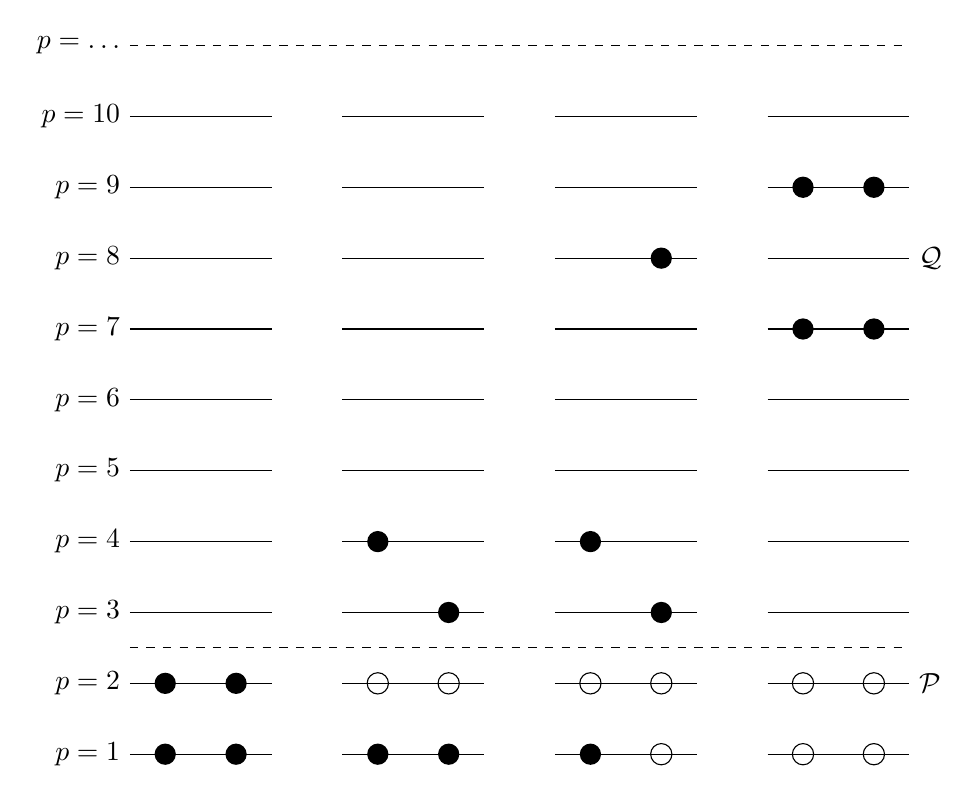
\begin{tikzpicture}[scale=0.9]
        % Draw lines
        \foreach \y in {1,2,...,10} {
            \draw (0, \y) -- (2, \y);
            \draw (3, \y) -- (5, \y);
            \draw (6, \y) -- (8, \y);
            \draw (9, \y) -- (11, \y);
            % \draw (12, \y) -- (14, \y);
        }
        % Draw additional dashed lines
        \draw[dashed] (0, 2.5) -- (11, 2.5);
        \draw[dashed] (0, 11) -- (11, 11);

        % Labels on the left
        \foreach \y/\label in {1/$p=1$, 2/$p=2$, 3/$p=3$, 4/$p=4$, 5/$p=5$, 6/$p=6$, 7/$p=7$, 8/$p=8$, 9/$p=9$, 10/$p=10$, 11/$p=\ldots$} {
            \node[left] at (0, \y) {\label};
        }

        % Labels on the right
        \node[right] at (11, 8) {$\mathcal{Q}$};
        \node[right] at (11, 2) {$\mathcal{P}$};

        % First 4-particle state
        \foreach \x/\y in {0.5/1, 0.5/2, 1.5/1, 1.5/2} {
            \fill (\x, \y) circle (0.15);
        }

        % Second 4-particle state
        \foreach \x/\y in {3.5/1, 4.5/1, 3.5/4, 4.5/3} {
            \fill (\x, \y) circle (0.15);
        }
        \foreach \x/\y in {3.5/2, 4.5/2} {
            \draw (\x, \y) circle (0.15);
        }

        % Third 4-particle state
        \foreach \x/\y in {6.5/1, 7.5/3, 6.5/4, 7.5/8} {
            \fill (\x, \y) circle (0.15);
        }
        \foreach \x/\y in {7.5/1, 6.5/2, 7.5/2} {
            \draw (\x, \y) circle (0.15);
        }

        % Fourth 4-particle state
        \foreach \x/\y in {9.5/7, 10.5/7, 9.5/9, 10.5/9} {
            \fill (\x, \y) circle (0.15);
        }
        \foreach \x/\y in {9.5/1, 10.5/1, 9.5/2, 10.5/2} {
            \draw (\x, \y) circle (0.15);
        }
    \end{tikzpicture}
    \caption{
        Schematic plot of the possible single-particle levels with double degeneracy.
        The filled circles indicate occupied particle states while the empty circles represent vacant particle (hole) states.
        The spacing between each level $p$ is constant in this picture.
        The first two single-particle levels define our possible model space, indicated by the label $\mathcal{P}$.
        The remaining states span the excluded space $\mathcal{Q}$.
        The first state to the left represents a possible ground state representation for a four-fermion system.
        In the second state to the left, one pair is broken.
        This possibility is however not included in our interaction.\label{fig:schematic}
    }
\end{figure}

\newpage
\section{}
Show that the unperturbed Hamiltonian $\hat{H}_0$ and $\hat{V}$ commute with both the spin projection $\hat{S}_z$ and the total spin $\hat{S}^2$, given by
\begin{equation*}
    \hat{S}_z := \frac{1}{2} \sum_{p\sigma} \sigma a^\dag_{p\sigma} a_{p\sigma} \quad \text{and} \quad \hat{S}^2 := \hat{S}_z^2 + \frac{1}{2}(\hat{S}_ + \hat{S}_ - + \hat{S}_ - \hat{S}_+),
\end{equation*}
where
\begin{equation*}
    \hat{S}_\pm := \sum_{p} a^\dag_{p\pm} a_{p\mp}.
\end{equation*}

This is an important feature of our system that allows us to block-diagonalize the full Hamiltonian.
We will focus on total spin $S=0$.
In this case, it is convenient to define the so-called pair creation and pair annihilation operators
\begin{equation*}
    \hat{P}^{+}_p = a^\dag_{p+} a^\dag_{p-} \quad \text{and} \quad \hat{P}^{-}_p = a_{p-} a_{p+},
\end{equation*}
respectively.

Show that you can rewrite the Hamiltonian (with $\xi=1$) as
\begin{equation*}
    \hat{H} = \sum_{p\sigma} (p-1) a_{p\sigma}^{\dagger} a_{p\sigma} - \frac{1}{2} g \sum_{pq} \hat{P}^{+}_p \hat{P}^{-}_q.
\end{equation*}
Show also that pair creation operators  commute among themselves.

In this midterm we focus only on a system with no broken pairs.
This means that the Hamiltonian can only link two-particle states in so-called spin-reversed states.

\subsection{}
We firstly need to show that the unperturbed Hamiltonian $\hat{H}_0$ and the two-body operator $\hat{V}$ commute with the spin projection $\hat{S}_z$.
We have, being careful with the summation indices,
\begin{align*}
    \left[ \hat{H}_0, \hat{S}_z \right]
    &= \left[
        \sum_{p\sigma} (p-1) a_{p\sigma}^{\dagger} a_{p\sigma},
        \frac{1}{2} \sum_{q\tau} \tau a^\dag_{q\tau} a_{q\tau}
    \right] \\
    &= \frac{1}{2} \sum_{p\sigma} (p-1) \sum_{q\tau} \tau \left[
        a_{p\sigma}^{\dagger} a_{p\sigma},
        a^\dag_{q\tau} a_{q\tau}
    \right] \\
    &= \frac{1}{2} \sum_{p\sigma} (p-1) \sum_{q\tau} \tau \left[
        \hat{n}_{p\sigma}, \hat{n}_{q\tau}
    \right],
\end{align*}
where we have defined the number operator $\hat{n}_{p\sigma} = a_{p\sigma}^{\dagger} a_{p\sigma}$.
As the number operator commutes with itself, we have that $\left[ \hat{n}_{p\sigma}, \hat{n}_{q\tau} \right] = 0$, and thus $[ \hat{H}_0, \hat{S}_z ] = 0$.

Next, we show that the two-body operator $\hat{V}$ commutes with the spin projection $\hat{S}_z$.
We have, again being careful with the summation indices,
\begin{align*}
    \left[ \hat{V}, \hat{S}_z \right]
    &= \left[
        -\frac{1}{2} g \sum_{pq} a_{p+}^\dagger a_{p-}^\dagger a_{q-} a_{q+},
        \frac{1}{2} \sum_{r\sigma} \sigma a^\dag_{r\sigma} a_{r\sigma}
    \right] \\
    &= -\frac{1}{4} g \sum_{pqr \sigma} \sigma \left[
        a_{p+}^\dagger a_{p-}^\dagger a_{q-} a_{q+},
        a^\dag_{r\sigma} a_{r\sigma}
    \right] \\
    &= -\frac{1}{4} g \sum_{pqr \sigma} \sigma \left[
        a_{p+}^\dagger a_{p-}^\dagger a_{q-} a_{q+},
        \hat{n}_{r\sigma}
    \right].
\end{align*}
Using the commutation indentity
\begin{equation*}
    \left[ AB, C \right] = A \left[B, C \right] + \left[ A, C \right] B,
\end{equation*}
we have
\begin{equation}\label{eq:double_comm}
    \left[ a_{p+}^\dagger a_{p-}^\dagger a_{q-} a_{q+}, \hat{n}_{r\sigma} \right]
    = a_{p+}^\dagger a_{p-}^\dagger \Big[ a_{q-} a_{q+}, \hat{n}_{r\sigma} \Big] + \left[ a_{p+}^\dagger a_{p-}^\dagger, \hat{n}_{r\sigma} \right] a_{q-} a_{q+},
\end{equation}
and then need to find expressions for
\begin{equation*}
    \Big[ a_{q-} a_{q+}, \hat{n}_{r\sigma} \Big] \quad \text{and} \quad \left[ a_{p+}^\dagger a_{p-}^\dagger, \hat{n}_{r\sigma} \right].
\end{equation*}

Changing the indices for brevity in the intermediate steps, we need to find
\begin{equation*}
    \left[ a_{p} a_{q}, \hat{n}_{r} \right] \quad \text{and} \quad \left[ a_{p}^\dagger a_{q}^\dagger, \hat{n}_{r} \right],
\end{equation*}
noting that
\begin{equation*}
    \left[ a_{p} a_{q}, \hat{n}_{r} \right]
    = a_{p} \left[ a_{q}, \hat{n}_{r} \right] + \left[ a_{p}, \hat{n}_{r} \right] a_{q}.
\end{equation*}
As
\begin{align*}
    \left[ a_q, \hat{n}_{r} \right] &= \left[ a_q, a_{r}^\dagger a_{r} \right]
    = \left[ a_q, a_{r}^\dagger \right] a_{r} + a_{r}^\dagger \left[ a_q, a_{r} \right] \\
    &= \delta_{qr} a_{r} + a_{r}^\dagger \cdot 0
    = \delta_{qr} a_{r} = a_{q},
\end{align*}
We have
\begin{align*}
    \left[ a_{p} a_{q}, \hat{n}_{r} \right]
    &= a_{p} \left[ a_{q}, \hat{n}_{r} \right] + \left[ a_{p}, \hat{n}_{r} \right] a_{q} \\
    &= a_{p} a_{q} + a_{p} a_{q} = 2 a_{p} a_{q}.
\end{align*}
Similarly, for the creation operators, we have
\begin{equation*}
    \left[ a_p^\dagger, \hat{n}_r \right] = \left[ a_p^\dagger, a_r^\dagger a_r \right] = \left[ a_p^\dagger, a_r^\dagger \right] a_r + a_r^\dagger \left[ a_p^\dagger, a_r \right] = -\delta_{pr} a_r^\dagger = -a_p^\dagger,
\end{equation*}
and thus
\begin{align*}
    \left[ a_p^\dagger a_q^\dagger, \hat{n}_r \right]
    &= a_p^\dagger \left[ a_q^\dagger, \hat{n}_r \right] + \left[ a_p^\dagger, \hat{n}_r \right] a_q^\dagger \\
    &= - a_p^\dagger a_q^\dagger - a_p^\dagger a_q^\dagger = - 2 a_p^\dagger a_q^\dagger.
\end{align*}

Returning to Eq.~\eqref{eq:double_comm} with the correct labels, we have
\begin{align*}
    \left[ a_{p+}^\dagger a_{p-}^\dagger a_{q-} a_{q+}, \hat{n}_{r\sigma} \right]
    &= a_{p+}^\dagger a_{p-}^\dagger \Big[ a_{q-} a_{q+}, \hat{n}_{r\sigma} \Big] + \left[ a_{p+}^\dagger a_{p-}^\dagger, \hat{n}_{r\sigma} \right] a_{q-} a_{q+} \\
    &= 2 a_{p+}^\dagger a_{p-}^\dagger a_{q-} a_{q+} - 2 a_{p+}^\dagger a_{p-}^\dagger a_{q-} a_{q+} \\
    &= 0,
\end{align*}
meaning that
\begin{align*}
    \left[ \hat{V}, \hat{S}_z \right] = -\frac{1}{4} g \sum_{pqr \sigma} \sigma \left[
        a_{p+}^\dagger a_{p-}^\dagger a_{q-} a_{q+},
        \hat{n}_{r\sigma}
    \right] = 0.
\end{align*}
We have thus shown that the unperturbed Hamiltonian $\hat{H}_0$ and the two-body operator $\hat{V}$ commute with the spin projection $\hat{S}_z$.

Next, we want to show the commutations of $\hat{H}_0$ and $\hat{V}$ with the total spin $\hat{S}^2$.
Starting with $\hat{H}_0$, we have
\begin{align*}
    \left[ \hat{H}_0, \hat{S}^2 \right]
    &= \left[
        \hat{H}_0,
        \hat{S}_z^2 + \frac{1}{2}(\hat{S}_+ \hat{S}_- + \hat{S}_- \hat{S}_+)
    \right] \\
    &= \left[ \hat{H}_0, \hat{S}_z^2 \right] + \left[ \hat{H}_0, \frac{1}{2}(\hat{S}_+ \hat{S}_- + \hat{S}_- \hat{S}_+) \right].
\end{align*}
As we have shown that $\hat{H}_0$ commutes with $\hat{S}_z$, we also have $\left[ \hat{H}_0, \hat{S}_z^2 \right] = 0$, and thus only need to place our attention on
\begin{align*}
    \left[ \hat{H}_0, \frac{1}{2}(\hat{S}_+ \hat{S}_- + \hat{S}_- \hat{S}_+) \right]
    &= \frac{1}{2} \left(
        \left[
            \hat{H}_0, \hat{S}_+ \hat{S}_-
        \right]
        + \left[
            \hat{H}_0, \hat{S}_- \hat{S}_+
        \right]
    \right).
\end{align*}
We will only show the commutation of $\hat{H}_0$ with $\hat{S}_{\pm} \hat{S}_{\mp}$.
Breaking the expression down further, we have
\begin{equation*}
    \left[ \hat{H}_0, \hat{S}_\pm \hat{S}_\mp \right]
    = \left[ \hat{H}_0, \hat{S}_\pm \right] \hat{S}_\mp + \hat{S}_\pm \left[ \hat{H}_0, \hat{S}_\mp \right].
\end{equation*}
We then have
\begin{align*}
    \left[ \hat{H}_0, \hat{S}_{\pm} \right]
    &= \left[
        \sum_{p\sigma} (p-1) a_{p\sigma}^{\dagger} a_{p\sigma},
        \sum_{q} a^\dag_{q\pm} a_{q\mp}
    \right] \\
    &= \sum_{pq \sigma} (p-1) \left[
        a_{p\sigma}^{\dagger} a_{p\sigma},
        a^\dag_{q\pm} a_{q\mp}
    \right].
\end{align*}
Considering the commutation, using the number operator, we have
\begin{align*}
    \left[ \hat{n}_{p\sigma}, a^\dag_{q\pm} a_{q\mp} \right]
    &= a^\dag_{q\pm} \left[ \hat{n}_{p\sigma}, a_{q\mp} \right] + \left[ \hat{n}_{p\sigma}, a^\dag_{q\pm} \right] a_{q\mp} \\
    &= - a^\dag_{q\pm} a_{q\mp} + a^\dag_{q\pm} a_{q\mp} = 0,
\end{align*}
and thus
\begin{equation*}
    \left[ \hat{H}_0, \hat{S}_{\pm} \right] = 0.
\end{equation*}
We have thus shown that $\left[ \hat{H}_0, \hat{S}^2 \right] = 0$.

Next, we show that $\hat{V}$ commutes with $\hat{S}^2$.
We have
\begin{align*}
    \left[ \hat{V}, \hat{S}^2 \right]
    &= \left[
        -\frac{1}{2} g \sum_{pq} a_{p+}^\dagger a_{p-}^\dagger a_{q-} a_{q+},
        \hat{S}_z^2 + \frac{1}{2}(\hat{S}_+ \hat{S}_- + \hat{S}_- \hat{S}_+)
    \right] \\
    &= \left[ \hat{V}, \hat{S}_z^2 \right] + \left[ \hat{V}, \frac{1}{2}(\hat{S}_+ \hat{S}_- + \hat{S}_- \hat{S}_+) \right].
\end{align*}
Again, as we've already shown that $\hat{V}$ commutes with $\hat{S}_z$, we only need to consider the commutation with $\hat{S}_\pm \hat{S}_\mp$.
We analogously again have
\begin{equation*}
    \left[ \hat{V}, \hat{S}_\pm \hat{S}_\mp \right]
    = \left[ \hat{V}, \hat{S}_\pm \right] \hat{S}_\mp + \hat{S}_\pm \left[ \hat{V}, \hat{S}_\mp \right],
\end{equation*}
where
\begin{align*}
    \left[ \hat{V}, \hat{S}_{\pm} \right]
    &= \left[
        -\frac{1}{2} g \sum_{pq} a_{p+}^\dagger a_{p-}^\dagger a_{q-} a_{q+},
        \sum_{r} a^\dag_{r\pm} a_{r\mp}
    \right] \\
    &= -\frac{1}{2} g \sum_{pqr} \left[
        a_{p+}^\dagger a_{p-}^\dagger a_{q-} a_{q+},
        a^\dag_{r\pm} a_{r\mp}
    \right].
\end{align*}
Breaking the expression down further, we have
\begin{equation}\label{eq:V_to_S_comm}
    \begin{split}
        \left[
            a_{p+}^\dagger a_{p-}^\dagger a_{q-} a_{q+},
            a^\dag_{r\pm} a_{r\mp}
        \right] &= a_{p+}^\dagger a_{p-}^\dagger \left[ a_{q-} a_{q+}, a^\dag_{r\pm} a_{r\mp} \right] \\
        &+ \left[ a_{p+}^\dagger a_{p-}^\dagger, a^\dag_{r\pm} a_{r\mp} \right] a_{q-} a_{q+}.
    \end{split}
\end{equation}
Considering the two contractions seperately, starting with the first one:
\begin{equation*}
    \left[ a_{q-} a_{q+}, a^\dag_{r\pm} a_{r\mp} \right]
    = a_{q-} \left[ a_{q+}, a^\dag_{r\pm} a_{r\mp} \right] + \left[ a_{q-}, a^\dag_{r\pm} a_{r\mp} \right] a_{q+}.
\end{equation*}
These expressions follow the same pattern, so we only consider $q \pm \mapsto q$.
\begin{align*}
    \left[ a_{q}, a^\dag_{r\pm} a_{r\mp} \right]
    &= \left[ a_q, a^\dag_{r\pm} \right] a_{r \mp} + a^\dag_{r\pm} \Big[ a_q, a_{r\mp} \Big] \\
    &= \delta_{q, r\pm} a_{r\mp} + a^\dag_{r\pm} \cdot 0 = \delta_{q, r\pm} a_{r\mp}.
\end{align*}
We thus only get a contribution when $q = r$ and the spin parities match.
We then have
\begin{align*}
    \left[ a_{q-} a_{q+}, a^\dag_{r\pm} a_{r\mp} \right]
    &= a_{q-} \left[ a_{q+}, a^\dag_{r\pm} a_{r\mp} \right] + \left[ a_{q-}, a^\dag_{r\pm} a_{r\mp} \right] a_{q+} \\
    &= a_{q-} \delta_{q+, r\pm} a_{r\mp} + \delta_{q-, r\pm} a_{r\mp} a_{q+} \\
    &= \delta_{q+, r\pm} a_{q-} a_{r\mp} - \delta_{q-, r\pm} a_{q+} a_{r\mp} \\
\end{align*}
Continuing with the second contraction, we have
\begin{equation*}
    \left[ a_{p+}^\dagger a_{p-}^\dagger, a^\dag_{r\pm} a_{r\mp} \right] = a_{p+}^\dagger \left[ a_{p-}^\dagger, a^\dag_{r\pm} a_{r\mp} \right] + \left[ a_{p+}^\dagger, a^\dag_{r\pm} a_{r\mp} \right] a_{p-}^\dagger,
\end{equation*}
which again follow the same pattern.
Writing $p \pm \mapsto p$ we have
\begin{align*}
    \left[ a_{p}^\dagger, a^\dag_{r\pm} a_{r\mp} \right]
    &= \left[ a_p^\dagger, a^\dag_{r\pm} \right] a_{r\mp} + a^\dag_{r\pm} \left[ a_p^\dagger, a_{r\mp} \right] \\
    &= 0 \cdot a_{r\mp} - a^\dag_{r\pm} \delta_{p, r\mp} = - a^\dag_{r\pm} \delta_{p, r\mp}.
\end{align*}
Inserting the expressions back into the commutator, we have
\begin{align*}
    \left[ a_{p+}^\dagger a_{p-}^\dagger, a^\dag_{r\pm} a_{r\mp} \right]
    &= a_{p+}^\dagger \left[ a_{p-}^\dagger, a^\dag_{r\pm} a_{r\mp} \right] + \left[ a_{p+}^\dagger, a^\dag_{r\pm} a_{r\mp} \right] a_{p-}^\dagger \\
    &= - a_{p+}^\dagger a^\dag_{r\pm} \delta_{p-, r\mp} - a^\dag_{r\pm} \delta_{p+, r\mp} a_{p-}^\dagger \\
    &= - \delta_{p-, r\mp} a_{p+}^\dagger a^\dag_{r\pm} + \delta_{p+, r\mp} a_{p-}^\dagger a^\dag_{r\pm}.
\end{align*}

As the results are getting quite wieldy, we summarize the different cases of spin parities in the commutator.
\begin{align*}
    \left[ a_{q-} a_{q+}, a^\dag_{r+} a_{r-} \right] &= \delta_{q+, r+} a_{q-} a_{r-} = 0 \\
    \left[ a_{q-} a_{q+}, a^\dag_{r-} a_{r+} \right] &= -\delta_{q-, r-} a_{q+} a_{r+} = 0 \\
    \left[ a_{p+}^\dagger a_{p-}^\dagger, a^\dag_{r+} a_{r-} \right] &= - \delta_{p-, r-} a_{p+}^\dagger a^\dag_{r+} = 0 \\
    \left[ a_{p+}^\dagger a_{p-}^\dagger, a^\dag_{r-} a_{r+} \right] &= \delta_{p+, r+} a_{p-}^\dagger a^\dag_{r-} = 0.
\end{align*}
We thus have that that Eq.~\eqref{eq:V_to_S_comm} simplifies to
\begin{equation*}
    \left[ a_{p+}^\dagger a_{p-}^\dagger a_{q-} a_{q+}, a^\dag_{r\pm} a_{r\mp} \right] = 0,
\end{equation*}
which means that $\left[ \hat{V}, \hat{S}_\pm \right] = 0$, giving us that
\begin{equation*}
    \left[ \hat{V}, \hat{S}^2 \right] = 0.
\end{equation*}
We have thus shown that both $\hat{H}_0$ and $\hat{V}$ commute with the total spin $\hat{S}^2$.

With $\xi = 1$, the one-body operator $\hat{H}_0$ is defined as
\begin{equation*}
    \hat{H}_0 = \sum_{p\sigma} (p-1) a_{p\sigma}^{\dagger} a_{p\sigma}.
\end{equation*}
For the two-body operator $\hat{V}$, we have, substituting $\hat{P}^{+}_p = a_{p+}^\dagger a_{p-}^\dagger$ and $\hat{P}^{-}_q = a_{q-} a_{q+}$,
\begin{equation*}
    \hat{V} = - \frac{1}{2} g \sum_{pq} \hat{P}^{+}_p \hat{P}^{-}_q.
\end{equation*}
This leaves us with the rewritten Hamiltonian
\begin{equation*}
    \hat{H} = \hat{H}_0 + \hat{V} = \sum_{p\sigma} (p-1) a_{p\sigma}^{\dagger} a_{p\sigma} - \frac{1}{2} g \sum_{pq} \hat{P}^{+}_p \hat{P}^{-}_q.
\end{equation*}

Finally, we want to show that the pair creation operators commute among themselves.
\begin{align*}
    \left[ \hat{P}^{+}_p, \hat{P}^{+}_q \right]
    &= \left[ a_{p+}^\dagger a_{p-}^\dagger, a_{q+}^\dagger a_{q-}^\dagger \right] \\
    &= a_{p+}^\dagger a_{p-}^\dagger a_{q+}^\dagger a_{q-}^\dagger - a_{q+}^\dagger a_{q-}^\dagger a_{p+}^\dagger a_{p-}^\dagger \\
    &= a_{p+}^\dagger a_{p-}^\dagger a_{q+}^\dagger a_{q-}^\dagger - (-1)^2 a_{p+}^\dagger a_{q+}^\dagger a_{q-}^\dagger a_{p-}^\dagger \\
    &= a_{p+}^\dagger a_{p-}^\dagger a_{q+}^\dagger a_{q-}^\dagger - (-1)^4 a_{p+}^\dagger a_{p-}^\dagger a_{q+}^\dagger a_{q-}^\dagger \\
    &= 0.
\end{align*}
Similarly, one can show that the pair annihilation operators also commute among themselves.


\newpage
\section{}
Define the Hamiltonian in a second-quantized form and use this to compute the expectation value of the ground state (defining the so-called reference energy and later our Hartree-Fock functional) of
the helium atom.
Show that it is given by
\begin{equation}
    E[\Phi_0] = \expval{c}{\hat{H}}{c} = \sum_{i} \expval{i}{\hat{h}_0}{i} + \frac{1}{2} \sum_{ij} \left[\expval*{ij}{\frac{1}{r_{ij}}}{ij} - \expval*{ij}{\frac{1}{r_{ij}}}{ji}\right].
\end{equation}
Define properly the sums keeping in mind that the states $ij$ refer to all quantum numbers $n, l, m_l, s, m_s$.
Use the values for the various matrix elements listed at the end of the midterm to find the value of $E$ as function of $Z$ and compute $E$ as function of $Z$.

\subsection{}
We consider the Hamiltonian $\hat{H} = \hat{H}_0 + \hat{H}_I$, where $\hat{H}_0$ is the one-body part and $\hat{H}_I$ is the two-body part, given by
\begin{align*}
    \hat{H}_0 &= \sum_{i=1}^{N}\hat{h}_0(x_i), &
    \hat{H}_I &= \sum_{i<j}^{N}\frac{1}{r_{ij}}.
\end{align*}
In second quantization, we rewrite the one-body part as
\begin{equation}
    \hat{H}_0 = \sum_{\alpha\beta} \expval{\alpha}{\hat{h}_0}{\beta} a_\alpha^\dagger a_\beta.
\end{equation}
Then, the expectation value of the ground state with the one-body part is given by
\begin{equation*}
    \expval{\Phi_0}{\hat{H}_0}{\Phi_0} = \sum_{\alpha\beta} \expval{\alpha}{\hat{h}_0}{\beta} \expval{\Phi_0}{a_\alpha^\dagger a_\beta}{\Phi_0}.
\end{equation*}
For all states where either $\alpha > F, \beta > F$, we have that $\expval{\Phi_0}{a_\alpha^\dagger a_\beta}{\Phi_0} = 0$.
Thus, the sum is restricted to $i,j \le F$,
\begin{align*}
    \expval{\Phi_0}{\hat{H}_0}{\Phi_0} &= \sum_{ij} \expval{i}{\hat{h}_0}{j} \expval{\Phi_0}{a_i^\dagger a_j}{\Phi_0} \\
    &= \sum_{ij} \expval{i}{\hat{h}_0}{j} \delta_{ij} \\
    &= \sum_{i} \expval{i}{\hat{h}_0}{i},
\end{align*}
where we utilized the orthonormality of the single-particle states.

The two-body part is rewritten in second quantization as
\begin{equation*}
    \hat{H}_I = \frac{1}{2} \sum_{\alpha \beta \gamma \delta} \expval{\alpha \beta}{V}{\gamma \delta} a_\alpha^\dagger a_\beta^\dagger a_\delta a_\gamma.
\end{equation*}
The expectation value of the ground state with the two-body part is then
\begin{equation*}
    \expval{\Phi_0}{\hat{H}_I}{\Phi_0} = \frac{1}{2} \sum_{\alpha\beta\gamma\delta} \expval{\alpha\beta}{V}{\gamma\delta} \expval{\Phi_0}{a_\alpha^\dagger a_\beta^\dagger a_\delta a_\gamma}{\Phi_0}.
\end{equation*}
The possible contributing contractions are
\begin{align*}
    \wick{\c2 a_\alpha^\dagger \c1 a_\beta^\dagger \c1 a_\delta \c2 a_\gamma} &= \delta_{\alpha\gamma} \delta_{\beta\delta}, &
    \wick{\c1 a_\alpha^\dagger \c2 a_\beta^\dagger \c1 a_\delta \c2 a_\gamma} &= -\delta_{\alpha\delta} \delta_{\beta\gamma}. \\
\end{align*}
Whenever $\alpha > F$ or $\beta > F$, the expectation value vanishes, so we relabel the summation to $i, j$. The terms also vanish if $i = j$. % TODO: Reword maybe
We are then left with
\begin{equation*}
    \expval{\Phi_0}{\hat{H}_0}{\Phi_0} = \frac{1}{2} \sum_{\substack{ij \\ i \neq j}} \expval*{ij}{V}{ij} - \expval*{ij}{V}{ji}.
\end{equation*}

Gathering this, we get that the complete expectation value of the ground state is
\begin{equation}
    E[\Phi_0]
    = \expval{c}{\hat{H}}{c}
    = \sum_{i} \expval{i}{\hat{h}_0}{i} + \frac{1}{2} \sum_{\substack{ij \\ i \neq j}} \expval*{ij}{\frac{1}{r_{ij}}}{ij} - \expval*{ij}{\frac{1}{r_{ij}}}{ji},
\end{equation}
as we wanted to show.

In the case of the electrons in the helium atom, we only have $n = 1$, $l = 0$, differing only in the spin quantum number $m_s = \pm 1/2$.
The expectation value of the one-body part is then
\begin{equation*}
    \expval{\Phi_0}{\hat{h}_0}{\Phi_0} = \sum_{\sigma \in \{\pm 1/2\}} \expval{1\sigma}{\hat{h}_0}{1\sigma} = -\frac{Z^2}{n^2},
\end{equation*}
and the expectation value of the two-body part is, writing just $\sigma_{+}$ and $\sigma_{-}$ for the spins,
\begin{equation*}
    \expval{\Phi_0}{\hat{H}_I}{\Phi_0}
    = \frac{1}{2} \sum_{\substack{\sigma_{+}\sigma_{-}\\ \sigma_{+} \neq \sigma_{-}}}
    \underbrace{\expval*{\sigma_{+} \sigma_{-}}{\frac{1}{r_{\sigma_{+}\sigma_{-}}}}{\sigma_{+} \sigma_{-}}}_{\textnormal{Direct term}}
    - \underbrace{\expval*{\sigma_{+} \sigma_{-}}{\frac{1}{r_{\sigma_{+}\sigma_{-}}}}{\sigma_{-}\sigma_{+}}}_{\textnormal{Exchange term}}.
\end{equation*}
The exchange term vanishes since the states are orthogonal, and we are left with the direct term.
We are then just left with
\begin{equation*}
    \expval{\Phi_0}{\hat{H}_I}{\Phi_0} = \frac{1}{2}\left[ \expval*{\sigma_{+} \sigma_{-}}{\frac{1}{r_{\sigma_{+} \sigma_{-}}}}{\sigma_{+} \sigma_{-}} + \expval*{\sigma_{-} \sigma_{+}}{\frac{1}{r_{\sigma_{+} \sigma_{-}}}}{\sigma_{-} \sigma_{+}}\right].
\end{equation*}
As $\hat{H}_I$ is invariant under the change of label $\sigma$, we can simplify this to
\begin{equation*}
    \expval{\Phi_0}{\hat{H}_I}{\Phi_0} = \expval*{\sigma_{+} \sigma_{-}}{\frac{1}{r_{\sigma_{+} \sigma_{-}}}}{\sigma_{+} \sigma_{-}}.
\end{equation*}

Computing this, we find that the expectation value of the ground state is
\begin{equation}
    E[\Phi_0] = -Z^2 + \tfrac{5}{8}Z,
\end{equation}
which as a function of $Z$ is shown in \autoref{fig:energy}.

\begin{figure}[ht]
    \centering
    \includegraphics{figs/energy_plot.pdf}
    \caption{The expectation value of the ground states of an atom with two electrons as a function of the nuclear charge $Z$.\label{fig:energy}}
\end{figure}


\newpage
\section{}
Hereafter we will limit ourselves to a system which now contains only one-particle-one-hole excitations beyond the chosen state $\ket{c}$.
Using the possible Slater determinants from exercise a) for the helium atom, find the expressions (without inserting the explicit values for the matrix elements first) for % chktex 10 % tex-fmt: skip
\begin{equation*}
    \expval{c}{\hat{H}}{\Phi_i^a},
\end{equation*}
and
\begin{equation*}
    \expval{\Phi_i^a}{\hat{H}}{\Phi_j^b}.
\end{equation*}
Represent these expressions in a diagrammatic form, both for the onebody part and the two-body part of the Hamiltonian.

Insert then the explicit values for the various matrix elements and set up the final Hamiltonian matrix and diagonalize it using for example Python as programming language.
Compare your results from those of exercise b) and comment your results. % chktex 10 % tex-fmt: skip

The exact energy with our Hamiltonian is $-2.9037$ atomic units for helium.
This value is also close to the experimental energy.

\subsection{}
We start by finding the value of the expression $\expval{c}{\hat{H}}{\Phi_i^a}$.
Writing out the terms, we have
\begin{align*}
    \expval{c}{\hat{H}}{\Phi_i^a} &= \expval{c}{\hat{H}_0 + \hat{H}_I}{\Phi_i^a} \\
    &= \expval{c}{\hat{H}_0}{\Phi_i^a} + \expval{c}{\hat{H}_I}{\Phi_i^a}.
\end{align*}
We can now read from Eq.~\eqref{eq:H0_second_quant} that the one-body part of the expression vanishes, either through an unmatched $b_\alpha^\dagger$ or simply $\braket{c}{\Phi_i^a} = 0$.
This gives us
\begin{equation}\label{eq:1p1h-ground-onebody}
    \expval{c}{\hat{H}_0}{\Phi_i^a} = 0.
\end{equation}

\begin{comment}
    Considering the one-body part, we have
    \begin{align*}
        \expval{c}{\hat{H}_0}{\Phi_i^a} &= \sum_{\alpha\beta} \expval{\alpha}{\hat{h}_0}{\beta} \expval{c}{a_\alpha^\dagger a_\beta}{\Phi_i^a} \\
        &= \sum_{\alpha\beta} \expval{\alpha}{\hat{h}_0}{\beta} \expval{c}{a_\alpha^\dagger a_\beta a_a^\dagger a_i}{c}. \\
    \end{align*}
    The only possible contraction is
    \begin{equation*}
        \langle
        \wick{
            c
            \vert
            \c2 a_\alpha^\dagger \c1 a_\beta \c1 a_a^\dagger \c2 a_i
            \vert
            c
        }
        \rangle,
    \end{equation*}
    such that $\alpha = i$ and $\beta = a$.
    The expectation value of the one-body part is then
    \begin{equation*}
        \expval{c}{\hat{H}_0}{\Phi_i^a} = \sum_{\alpha \beta} \expval{\alpha}{\hat{h}_0}{\beta} \delta_{\alpha i} \delta_{\beta a} = \expval{i}{\hat{h}_0}{a} = 0,
    \end{equation*}
    which vanishes due to the $\delta_{ij}$ term of Eq.~\eqref{eq:onebody}.
\end{comment}

In order to make sure the number of annihilation and creation terms are correct, the contributing terms from $H_I$ are those with two more annihilation operators than creation operators, while also matching the number of holes and particles created.
We can then quickly reduce the possible contributing candidates to
\begin{equation*}
    \frac{1}{4} \sum_{aijk} \expval{ji}{V}{ak} b_k^\dagger b_j b_i b_a, \qquad
    \frac{1}{2} \sum_{aij} \expval{ji}{V}{ai} b_j b_a, \qquad
    \text{and} \qquad \mathcal{E}_I^\text{Ref}.
\end{equation*}
On closer inspection, we see that the first term vanishes, as $b_k^\dagger$ is unmatched, while the last term vanished due to $\braket{c}{\Phi_i^a} = 0$.

We then just need to evaluate the contractions of the second term, changing the labels of the sum $(a, i, j) \mapsto (b, j, k)$ to avoid confusion with $\ket{\Phi_i^a}$, which simply is
\begin{equation*}
    \langle c \vert
    \wick{
        \c2 b_k \c1 b_b \c1 b_a^\dagger \c2 b_i^\dagger
    }
    \vert c \rangle
    = \delta_{ik} \delta_{ab}.
\end{equation*}
We then get
\begin{equation}\label{eq:1p1h-ground-twobody}
    \expval*{c}{\hat{H}_I}{\Phi_i^a} = \frac{1}{2} \sum_{j} \expval{i j}{V}{a j}_{AS},
\end{equation}
taking into account that the matrix element in the sum is antisymmetrized.
Combining Eqs.~\eqref{eq:1p1h-ground-onebody}~and~\eqref{eq:1p1h-ground-twobody}, we get the final expression is
\begin{equation}\label{eq:1p1h-ground}
    \expval{c}{\hat{H}}{\Phi_i^a} = \frac{1}{2} \sum_{j \neq i} \expval{i j}{V}{a j} - \expval{i j}{V}{j a}.
\end{equation}

Finally, taking into account spin, the values we get for the one-particle-one-hole excitations are listed in Eq.~\eqref{eq:1p1h-ground-list}, with the only possible value for $j$ in each case of Eq.~\eqref{eq:1p1h-ground} listed to the far left.
For brevity, we write $j\sigma_{\pm}$ as just $j_{\pm}$ here.
\begin{equation}\label{eq:1p1h-ground-list}
    \arraycolsep=1.4pt
    \begin{array}{crcl}
        j = 1_{-}: \quad
        & \expval*{c}{\hat{H}}{\Phi_{1_{+}}^{2_{+}}}\hspace{0.27pt}
        & = &
        \expval{1_{-} 1_{+}}{V}{1_{-} 2_{+}} - \expval{1_{-} 1_{+}}{V}{2_{+} 1_{-}} \\

        j = 1_{-}: \quad
        & \expval*{c}{\hat{H}}{\Phi_{1_{+}}^{2_{+}}}\hspace{0.27pt}
        & = &
        \expval{1_{-} 1_{+}}{V}{1_{-} 3_{+}} - \expval{1_{-} 1_{+}}{V}{3_{+} 1_{-}} \\

        j = 1_{+}: \quad
        & \expval*{c}{\hat{H}}{\Phi_{1_{-}}^{2_{-}}}
        & = &
        \expval{1_{+} 1_{-}}{V}{1_{+} 2_{-}} - \expval{1_{+} 1_{-}}{V}{2_{-} 1_{+}} \\

        j = 1_{+}: \quad
        & \expval*{c}{\hat{H}}{\Phi_{1_{-}}^{3_{-}}}
        & = &
        \expval{1_{+} 1_{-}}{V}{1_{+} 3_{-}} - \expval{1_{+} 1_{-}}{V}{3_{-} 1_{+}}
    \end{array}
\end{equation}

\begin{comment}
    \newpage

    For the two-body part, writing $V$ for the two-particle operator, we have
    \begin{align*}
        \expval{c}{\hat{H}_I}{\Phi_i^a} &= \frac{1}{2} \sum_{\alpha\beta\gamma\delta} \expval{\alpha\beta}{V}{\gamma\delta} \expval{c}{a_\alpha^\dagger a_\beta^\dagger a_\delta a_\gamma}{\Phi_i^a} \\
        &= \frac{1}{2} \sum_{\alpha\beta\gamma\delta} \expval{\alpha\beta}{V}{\gamma\delta} \expval{c}{a_\alpha^\dagger a_\beta^\dagger a_\delta a_\gamma a_a^\dagger a_i}{c}.
    \end{align*}
    The possible contractions are then
    \begin{align*}
        \expval{\alpha\beta}{V}{\gamma\delta} \langle
        \wick{
            c
            \vert
            \c3 a_\alpha^\dagger \c2 a_\beta^\dagger \c1 a_\delta \c3 a_\gamma \c1 a_a^\dagger \c2 a_i
            \vert
            c
        }
        \rangle
        &= \delta_{\alpha \gamma} \delta_{\beta i} \delta_{\delta a} \expval{\alpha\beta}{V}{\gamma\delta}
        = \expval{\alpha i}{V}{\alpha a}, \\
        \expval{\alpha\beta}{V}{\gamma\delta} \langle
        \wick{
            c
            \vert
            \c3 a_\alpha^\dagger \c2 a_\beta^\dagger \c3 a_\delta \c1 a_\gamma \c1 a_a^\dagger \c2 a_i
            \vert
            c
        }
        \rangle
        &= -\delta_{\alpha \delta} \delta_{\beta i} \delta_{\gamma a} \expval{\alpha\beta}{V}{\gamma\delta} = -\expval{\alpha i}{V}{a \alpha}, \\
        \expval{\alpha\beta}{V}{\gamma\delta} \langle
        \wick{
            c
            \vert
            \c3 a_\alpha^\dagger \c2 a_\beta^\dagger \c1 a_\delta \c2 a_\gamma \c1 a_a^\dagger \c3 a_i
            \vert
            c
        }
        \rangle
        &= -\delta_{\alpha i} \delta_{\beta \gamma} \delta_{a \delta} \expval{\alpha\beta}{V}{\gamma\delta} = -\expval{i \beta}{V}{\beta a}, \\
        \expval{\alpha\beta}{V}{\gamma\delta} \langle
        \wick{
            c
            \vert
            \c2 a_\alpha^\dagger \c1 a_\beta^\dagger \c1 a_\delta \c1 a_\gamma \c1 a_a^\dagger \c2 a_i
            \vert
            c
        }
        \rangle
        &= \delta_{\alpha i} \delta_{\beta \delta} \delta_{\gamma a} \expval{\alpha\beta}{V}{\gamma\delta} = \expval{i \beta}{V}{a \beta}.
    \end{align*}
    Using the general fact that $\expval{\alpha \beta}{V}{\gamma \delta} = \expval{\beta \alpha}{V}{\delta \gamma}$, we can gather these terms into a single term
    % TODO: FIX OSKAR, gjør greia di
    % TODO: Commutation relations
    % TODO: Diagrams
    \begin{equation*}
        \expval{c}{\hat{H}_I}{\Phi_i^a} = \sum_{\alpha} \expval{\alpha i}{V}{\alpha a} - \expval{\alpha i}{V}{a \alpha}.
    \end{equation*}

    The final expression for the expectation value of the Hamiltonian between the ground state and a one-particle-one-hole excitation is then
    \begin{equation}\label{eq:1p1h-exp}
        \expval{c}{\hat{H}}{\Phi_i^a} = \expval{c}{\hat{H}_0}{\Phi_i^a} + \expval{c}{\hat{H}_I}{\Phi_i^a} = 0 + \sum_{\alpha} \expval{\alpha i}{V}{\alpha a} - \expval{\alpha i}{V}{a \alpha}.
    \end{equation}

    Finally, the values we get for the one-particle-one-hole excitations are listed in Eq.~\eqref{eq:1p1h-exp-list}, with the only possible value for $\alpha$ in each case of Eq.~\eqref{eq:1p1h-exp} listed to the far left.
    For brevity, we write $\beta\sigma_{\pm}$ as just $\beta_{\pm}$ here.
    \begin{equation}\label{eq:1p1h-exp-list}
        \arraycolsep=1.4pt % TODO: Fiks off-by-one pixel Oskar
        \begin{array}{crcl}
            \alpha = 1_{-}: \quad
            & \expval*{c}{\hat{H}}{\Phi_{1_{+}}^{2_{+}}}
            & = &
            \expval{1_{-} 1_{+}}{V}{1_{-} 2_{+}} - \expval{1_{-} 1_{+}}{V}{2_{+} 1_{-}} \\

            \alpha = 1_{-}: \quad
            & \expval*{c}{\hat{H}}{\Phi_{1_{+}}^{2_{+}}}
            & = &
            \expval{1_{-} 1_{+}}{V}{1_{-} 3_{+}} - \expval{1_{-} 1_{+}}{V}{3_{+} 1_{-}} \\

            \alpha = 1_{+}: \quad
            & \expval*{c}{\hat{H}}{\Phi_{1_{-}}^{2_{-}}}
            & = &
            \expval{1_{+} 1_{-}}{V}{1_{+} 2_{-}} - \expval{1_{+} 1_{-}}{V}{2_{-} 1_{+}} \\

            \alpha = 1_{+}: \quad
            & \expval*{c}{\hat{H}}{\Phi_{1_{-}}^{3_{-}}}
            & = &
            \expval{1_{+} 1_{-}}{V}{1_{+} 3_{-}} - \expval{1_{+} 1_{-}}{V}{3_{-} 1_{+}}
        \end{array}
    \end{equation}
\end{comment}

Next, we find a simplified expression for $\expval{\Phi_i^a}{\hat{H}}{\Phi_j^b}$,
noting that
\begin{equation*}
    \expval{\Phi_i^a}{\hat{H}}{\Phi_j^b} = \expval{c}{b_i b_a \hat{H} b_b^\dagger b_j^\dagger}{c}.
\end{equation*}
The possible contributing terms must then have an equal number of annihilation and creation operators in order to not vanish, reducing the candidates to
% \begin{enumerate}
%     \item $\displaystyle\frac{1}{4} \sum_{abcd} \expval{ab}{V}{cd} b_a^\dagger b_b^\dagger b_d b_c$
%     \item $\displaystyle\frac{1}{2} \sum_{abij} \expval{ai}{V}{bj} b_a^\dagger b_j^\dagger b_b b_i$
%     \item $\displaystyle\frac{1}{2} \sum_{abi} \expval{ai}{V}{bi} b_a^\dagger b_b$
%     \item $\displaystyle\frac{1}{4} \sum_{ijkl} \expval{kl}{V}{ij} b_i^\dagger b_j^\dagger b_l b_k$
%     \item $\displaystyle\frac{1}{2} \sum_{ijkl} \expval{ij}{V}{kj} b_k^\dagger b_i$
%     \item $\displaystyle\mathcal{E}_I^\text{Ref}$
% \end{enumerate}
\begin{equation*} % TODO: Fix formattering Oskar
    \begin{array}{cccccc}
        \displaystyle\frac{1}{4} \sum_{abcd} \expval{ab}{V}{cd} b_a^\dagger b_b^\dagger b_d b_c &, &
        \displaystyle\frac{1}{2} \sum_{abij} \expval{ai}{V}{bj} b_a^\dagger b_j^\dagger b_b b_i &, &
        \displaystyle\frac{1}{2} \sum_{abi} \expval{ai}{V}{bi} b_a^\dagger b_b, \\
        \displaystyle\frac{1}{4} \sum_{ijkl} \expval{kl}{V}{ij} b_i^\dagger b_j^\dagger b_l b_k &, &
        \displaystyle\frac{1}{2} \sum_{ijk} \expval{ij}{V}{kj} b_k^\dagger b_i &, &
        \displaystyle\mathcal{E}_I^\text{Ref}.
    \end{array}
\end{equation*}

% TODO: Bra nok formattering?
\begin{multicols}{2}{}
    \begin{enumerate}
        \item  $\displaystyle\frac{1}{4} \sum_{abcd} \expval{ab}{V}{cd} b_a^\dagger b_b^\dagger b_d b_c$
        \item  $\displaystyle\frac{1}{2} \sum_{abij} \expval{ai}{V}{bj} b_a^\dagger b_j^\dagger b_b b_i$
        \item  $\displaystyle\frac{1}{2} \sum_{abi} \expval{ai}{V}{bi} b_a^\dagger b_b$
        \item  $\displaystyle\frac{1}{4} \sum_{ijkl} \expval{kl}{V}{ij} b_i^\dagger b_j^\dagger b_l b_k$
        \item  $\displaystyle\frac{1}{2} \sum_{ijk} \expval{ij}{V}{kj} b_k^\dagger b_i$
        \item  $\displaystyle\mathcal{E}_I^\text{Ref}.$
    \end{enumerate}
\end{multicols}

For the terms here, recall that $\wick{\langle c \vert \c1 b_\alpha^\dagger \c1 b_\beta \vert c \rangle} = \delta_{\alpha \beta}$, while $\wick{\langle c \vert \c1 b_\alpha \c1 b_\beta^\dagger \vert c \rangle} = 0$.
The first term vanishes as $b_d b_c\ket{\Phi_j^{b}} =  \underbrace{b_d b_c b_b^\dagger b_j^†}_{0}\ket{c}= 0$, due to over-annihilation of particles.
For the second term, relabeling $(a, b, i, j) \mapsto (c, d, k, l)$ we get
\begin{equation*}
    \wick{
        \langle
        c \vert
        \c2 b_i
        \c1 b_a
        \c1 b_c^\dagger
        \c2 b_l^\dagger
        \c1 b_d
        \c2 b_k
        \c1 b_b^\dagger
        \c2 b_j^\dagger
        \vert c
        \rangle
    } = -\delta_{il} \delta_{ac} \delta_{db} \delta_{kj} \implies \frac{1}{2} \sum
\end{equation*}
\begin{comment}
    \begin{align*}
        \wick{
            \langle
            c \vert
            \c2 b_i
            \c1 b_a
            \underbrace{
                b_c^\dagger
                b_l^\dagger
                b_d
                b_k
            }_{\text{vanishes}}
            \c1 b_b^\dagger
            \c2 b_j^\dagger
            \vert c
            \rangle
        } &= 0, &
        \wick{
            \langle
            c \vert
            \c2 b_i
            \c1 b_a
            \c1 b_c^\dagger
            \c2 b_l^\dagger
            \c1 b_d
            \c2 b_k
            \c1 b_b^\dagger
            \c2 b_j^\dagger
            \vert c
            \rangle
        } &= -\delta_{il} \delta_{ac} \delta_{db} \delta_{kj}.
    \end{align*}
\end{comment}
For the third term, relabeling $(a, b, i) \mapsto (c, d, k)$, we have
\begin{equation*}
    \wick{
        \langle
        c \vert
        \c2 b_i
        \c1 b_a
        \c1 b_c^\dagger
        \c1 b_d
        \c1 b_b^\dagger
        \c2 b_j^\dagger
        \vert c
        \rangle
    } = \delta_{ij} \delta_{ab} \delta_{cd}.
\end{equation*}
The fourth term vanishes as the number of hole annihilation operator to the left of the creation operators does not match.
The fifth term, relabeling $(i, j, k) \mapsto (k, l, m)$, gives
\begin{equation*}
    \wick{
        \langle
        c \vert
        \c1 b_i
        \c2 b_a
        \c1 b_m^\dagger
        \c1 b_k
        \c2 b_b^\dagger
        \c1 b_j^\dagger
        \vert c
        \rangle
    } = \delta_{im} \delta_{ab} \delta_{kj}.
\end{equation*}
The last term simply gives us $\delta_{ab} \delta_{ij}$.

\newpage

Next, we find the expectation value of the Hamiltonian between two one-particle-one-hole excitations.
Considering the one-body part, we have
\begin{align*}
    \expval{\Phi_i^a}{\hat{H}_0}{\Phi_j^b} &= \sum_{\alpha\beta} \expval{\alpha}{\hat{h}_0}{\beta} \expval{\Phi_i^a}{a_\alpha^\dagger a_\beta}{\Phi_j^b} \\
    &= \sum_{\alpha\beta} \expval{\alpha}{\hat{h}_0}{\beta} \expval{c}{a_i^\dagger a_a  a_\alpha^\dagger a_\beta a_b^\dagger a_j}{c}.
\end{align*}
Note that if $\alpha > F$ or $\beta > F$, the expectation value vanishes.

The contractions are then
\begin{equation*}
    \arraycolsep=1.4pt
    \begin{array}{rlrcr}
        \expval{\alpha}{\hat{h}_0}{\beta}
        \langle
        \wick{
            c
            \vert
            \c2 a_i^\dagger \c1 a_a \c1 a_\alpha^\dagger \c1 a_\beta \c1 a_b^\dagger \c2 a_j
            \vert
            c
        }
        \rangle
        &=& \delta_{ij} \delta_{a \alpha} \delta_{b \beta} \expval{\alpha}{\hat{h}_0}{\beta}
        &=& \delta_{ij} \expval{a}{\hat{h}_0}{b} \,
        \\
        \expval{\alpha}{\hat{h}_0}{\beta}
        \langle
        \wick{
            c
            \vert
            \c1 a_i^\dagger \c2 a_a \c3 a_\alpha^\dagger \c1 a_\beta \c2 a_b^\dagger \c3 a_j
            \vert
            c
        }
        \rangle
        &= &- \delta_{i \beta} \delta_{a b} \delta_{\alpha j} \expval{\alpha}{\hat{h}_0}{\beta}
        &=& -\delta_{ab} \expval{j}{\hat{h}_0}{i} \;  \\
        \expval{\alpha}{\hat{h}_0}{\beta}
        \langle
        \wick{
            c
            \vert
            \c3 a_i^\dagger \c2 a_a \c1 a_\alpha^\dagger \c1 a_\beta \c2 a_b^\dagger \c3 a_j
            \vert
            c
        }
        \rangle
        &=& \delta_{i j} \delta_{a b} \delta_{\alpha \beta} \expval{\alpha}{\hat{h}_0}{\beta}
        &=& \delta_{i j} \delta_{a b} \expval{\alpha}{\hat{h}_0}{\alpha} \\
    \end{array}
\end{equation*}
meaning that the expectation value of the one-body part is
\begin{equation*}
    \expval{\Phi_i^a}{\hat{H}_0}{\Phi_j^b} = \delta_{ij} \expval{a}{\hat{h}_0}{b} - \delta_{ab} \expval{j}{\hat{h}_0}{i} + \delta_{ij} \delta_{ab} \sum_{\alpha \leq F} \expval{\alpha}{\hat{h}_0}{\alpha},
\end{equation*}
where we recognize the right-most term as the expectation value of the one-body operator in the ground state, known as the reference energy $\mathcal{E}_0^{\text{Ref}}$.
The term then vanishes whenever $i \neq j$ or $a \neq b$.

For the two-body part, we have
\begin{align*}
    \expval{\Phi_i^a}{\hat{H}_I}{\Phi_j^b} &= \frac{1}{2} \sum_{\alpha\beta\gamma\delta} \expval{\alpha\beta}{V}{\gamma\delta} \expval{\Phi_i^a}{a_\alpha^\dagger a_\beta^\dagger a_\delta a_\gamma}{\Phi_j^b} \\
    &= \frac{1}{2} \sum_{\alpha\beta\gamma\delta} \expval{\alpha\beta}{V}{\gamma\delta} \expval{c}{a_i^\dagger a_a a_\alpha^\dagger a_\beta^\dagger a_\delta a_\gamma a_b^\dagger a_j}{c}.  \\
\end{align*}
The possible contractions are then



\newpage
\section{}
We repeat parts b) and c) but now for the beryllium atom. % chktex 10 % tex-fmt: skip

Define the ansatz for $\ket{c}$ and limit yourself again to one-particle-one-hole excitations.
Compute the reference energy $\expval{c}{\hat{H}}{c}$ as function of $Z$.
Thereafter you will need to set up the appropriate Hamiltonian matrix which involves also one-particle-one-hole excitations.
Diagonalize this matrix and compare your eigenvalues with $\expval{c}{\hat{H}}{c}$ as function of $Z$ and comment your results.
The exact energy with our Hamiltonian is $-14.6674$ atomic units for beryllium.
This value is again close to the experimental energy.

With a given energy functional, we can perform at least two types of variational strategies.
These are:
\begin{enumerate}
    \item Vary the Slater determinant by changing the spatial part of the single-particle wave functions themselves, or

    \item Expand the single-particle functions in a known basis  and vary the coefficients, that is, the new function single-particle wave function $\ket{p}$ is written as a linear expansion in terms of a fixed basis $\phi$ (harmonic oscillator, Laguerre polynomials etc)
        \begin{equation*}
            \psi_p  = \sum_{\lambda} C_{p\lambda}\phi_{\lambda}
        \end{equation*}
\end{enumerate}
Both cases lead to a new Slater determinant which is related to the previous via a unitary transformation.
Below we will set up the Hartree-Fock equations using the second option.
We assume that our basis is still formed by the hydrogen-like wave functions.
We consider a Slater determinant built up of single-particle orbitals $\phi_{\lambda}$ where the indices $\lambda$ refer to specific single-particle states.
As an example, you could think of the ground state ansatz for the beryllium atom.

The unitary transformation
\begin{equation*}
    \psi_p  = \sum_{\lambda} C_{p\lambda}\phi_{\lambda},
\end{equation*}
brings us into the new basis $\psi$.
The new basis is orthonormal and $C$ is a unitary matrix.


\end{document} % chktex 17
